% !TeX root = er.tex

\chapter{Local Navigation: Obstacle Avoidance}\label{ch.obstacle}

\abstract*{A mobile robot navigating to a goal will encounter obstacles that must be avoided. Obstacle avoidance is presented in the context of wall following: moving around the wall of the obstacle until it no longer prevents access to the goal. Three algorithms are presented: simple wall following which fails in the presence of multiple obstacles, wall following with direction that also fails for certain obstacles and the Pledge algorithm which can avoid these obstacles. To demonstrate finding a path to a goal, an algorithm is presented that is based upon the behavior of a colony of ants searching for a food source even though they do not know its location. A probabilistic model explains the success of the algorithm.}

A mobile robot must \emph{navigate} from one point to another in its environment. This can be a simple task, for example, if a robot can follow an unobstructed line on the floor of a warehouse (Sect.~\ref{s.line}), but the task becomes more difficult in unknown and complex environments like a rover exploring the surface of Mars or a submersible exploring an undersea mountain range. Even a self-driving car which travels along a road needs to cope with other cars, obstacles on the road, pedestrian crosswalks, road construction, and so on. 

The navigation of a self-driving car can be divided into two tasks: There is the high-level task of finding a path between a starting position and a goal position. Before the development of modern computer systems, finding a path required you to study a map or to ask directions. Now there are smartphone applications which take a starting position and a goal position and compute paths between the two positions. If the application receives real-time data on traffic conditions, it can suggest which path will get you to your goal in the shortest time. The path can be computed offline, or, if you have a GPS system that can determine your current position, the path can be found in real-time and updated to take changing conditions into account.

A self-driving car must also perform the lower-level task of adapting its behavior to the environment: stopping for a pedestrian in a crosswalk, turning at intersections, avoiding obstacles in the road, and so on. While high-level path finding can be done once before the trip (or every few minutes), the low-level task of obstacle avoidance must be performed frequently, because the car never knows when a pedestrian will jump into the road or when the car it is following will suddenly brake.

Section~\ref{s.obstacle-avoidance} looks at the low-level task of obstacle avoidance. Section~\ref{s.no-localization} shows how a robot can recognize markings while following a line so that it knows when it has reached its goal. Sections~\ref{s.ants}--\ref{s.fsm-ants} demonstrate a higher-level behavior: finding a path without a map of the environment. This is done by analogy with a colony of ants locating a food source and communicating its location to all members of the colony.

\section{Obstacle avoidance}\label{s.obstacle-avoidance}
\index{obstacle avoidance}

The algorithms presented so far have focused on detecting objects and moving towards them. When a robot moves toward a goal it is likely to encounter additional objects called \emph{obstacles} that block the path and prevent the robot from reaching its goal. We assume that the robot is able to detect if there is an unobstructed path to the goal, for example, by detecting a light on the goal. This section describes three algorithms for obstacle avoidance, where the obstacles are walls that block the robot's movement:
\begin{itemize}
\item A straightforward wall following algorithm, which unfortunately will not work if there are multiple obstacles in the environment.
\item An algorithm that can avoid multiple obstacles, but it must know the general direction of the goal (perhaps from its GPS system). Unfortunately, some obstacles can cause the robot to become trapped in a loop.
\item The Pledge algorithm is a small modification of the second one that overcomes this erroneous behavior.
\end{itemize}
The algorithms will use the abstract conditional expressions \p{wall-ahead} and \p{wall-right}, which are true if there is a wall close to the front or to the right of the robot. The first algorithm will also use the conditional expression \p{corner-right} which is true if the robot is moving around an obstacle and senses a corner to its right. There are several ways of implementing these expressions which we pursue in Activity~\ref{act.wall-expressions}.

\begin{framed}
\act{Conditional expressions for wall following}{wall-expressions}
\begin{itemize}
\item Implement the conditional expression \p{wall-ahead} using a horizontal proximity or a touch sensor.
\item Implement the conditional expression \p{wall-right}. This is easy to do with a sensor mounted on the right of the robot, or with a rotating distance sensor. If you have only a forward-facing proximity sensor, you can have the robot turn slightly to the right, detect the wall, if any, and then turn back again.
\item Implement the conditional expression \p{corner-right}. This can be implemented as an extension of \p{wall-right}. When the value of \p{wall-right} changes from true to false, make a short right turn and check if \p{wall-right} becomes true again.
\end{itemize}
\end{framed}

\subsection{Wall following}
\index{wall following}

Figure~\ref{fig.wall-following-simple} shows a robot performing wall following by maintaining its position so that the wall is to its right (Algorithm~\ref{alg.wall-following-simple}). If a wall is detected ahead, the robot turns left so that the wall is to its right. If a wall is detected to the right, the robot continues moving along the wall. If a corner is detected, the robot turns right to continue moving around the obstacle. At the same time, the robot continually searches for the goal (black dot). When it detects the goal the robot moves directly towards it.

\begin{figure}
\begin{center}
\begin{tikzpicture}[scale=.7]
\draw[fill,color=gray] (4,0) rectangle +(4,.8);
\draw[fill,color=gray] (5,0) rectangle +(.8,-1);
\pic[rotate=90,scale=.5] at (7,-3) { robot };
\draw[fill] (6,4) node[right,xshift=4pt] {\p{Goal}} circle[radius=4pt];
\draw[->] (7,-2) -- ++(90:1.8) -- ++(180:1) -- ++(-90:1) -- ++(180:1.2) -- ++(90:1) -- ++(180:1) -- ++(90:1.2) coordinate(corner);
\draw[dashed,->] (corner) -- (5.9,3.9);
\path (-.3,0);  % Extra space so arrow isn't chopped
\end{tikzpicture}
\caption{Wall following}\label{fig.wall-following-simple}
\end{center}
\end{figure}

\begin{figure}
\begin{alg}{Simple wall following}{wall-following-simple}
\hline
\stl{}&while not-at-goal&\\
\stl{}&\idc{}if goal-detected&\\
\stl{}&\idc{}\idc{}move towards goal&\\
\stl{}&\idc{}else if wall-ahead&\\
\stl{}&\idc{}\idc{}turn left&\\
\stl{}&\idc{}else if corner-right&\\
\stl{}&\idc{}\idc{}turn right&\\
\stl{}&\idc{}else if wall-right&\\
\stl{}&\idc{}\idc{}move forward&\\
\stl{}&\idc{}else&\\
\stl{}&\idc{}\idc{}move forward&\\
\end{alg}
\end{figure}

Unfortunately, Algorithm~\ref{alg.wall-following-simple} does not always work correctly. Fig.~\ref{fig.wall-following-simple-bug} shows a configuration with \emph{two} obstacles between the robot and the goal. The robot will never detect the goal so it will move around the first obstacle indefinitely.

\begin{framed}
\act{Simple wall following}{simple-wall-following}
\begin{itemize}
\item Implement Algorithm~\ref{alg.wall-following-simple} and verify that it demonstrates the behaviors shown in Figs.\ref{fig.wall-following-simple}, \ref{fig.wall-following-simple-bug}.\
\end{itemize}
\end{framed}

\begin{figure}
\begin{center}
\begin{tikzpicture}[scale=.8]
\draw[fill,color=gray] (4,0) rectangle +(4,.8);
\draw[fill,color=gray] (5,0) rectangle +(.8,-1);
\draw[fill,color=gray] (0,2) rectangle +(9,.8);
\draw[fill,color=gray] (1.5,2) rectangle +(.8,-1);
\pic[rotate=90,scale=.5] at (7,-3) { robot };
\draw[fill] (6,4) node[right,xshift=4pt] {\p{Goal}} circle[radius=4pt];
\draw[->] (7,-2) -- ++(90:1.8) -- ++(180:1) -- ++(-90:1) -- ++(180:1.2) -- ++(90:1) -- ++(180:1) -- ++(90:1.2) coordinate(corner) -- ++(0:4.4) -- ++(-90:1.2) -- ++(180:1);
\draw[dashed,->] (corner) -- (5.9,3.9);
\path (-.3,0);  % Extra space so arrow isn't chopped
\end{tikzpicture}
\caption{Simple wall following doesn't always enable the robot to reach the goal}\label{fig.wall-following-simple-bug}
\end{center}
\end{figure}

\subsection{Wall following with direction}
\index{wall following!direction@with direction}

The problem with Algorithm~\ref{alg.wall-following-simple} is that it is a local algorithm that only looks at its immediate environment and does not take account of the fact that the higher-level navigation algorithm knows roughly the direction the robot should take to reach the goal. Figure~\ref{fig.wall-following-direction} shows the behavior of a robot that ``knows'' that the goal is somewhere to its north so the robot moves at a heading of $0^\circ$ relative to north. The wall following algorithm is only used if the robot cannot move north.

\begin{figure}
\begin{center}
\begin{tikzpicture}[scale=.7]
\draw[fill,color=gray] (4,0) rectangle +(4,.8);
\draw[fill,color=gray] (5,0) rectangle +(.8,-1);
\draw[fill,color=gray] (0,2) rectangle +(9,.8);
\draw[fill,color=gray] (1.5,2) rectangle +(.8,-1);
\pic[rotate=90,scale=.5] at (7,-3) { robot };
\draw[fill] (6,4) node[right,xshift=4pt] {\p{Goal}} circle[radius=4pt];
\draw[->] (7,-2) -- ++(90:1.8) -- ++(180:1) -- ++(-90:1) -- ++(180:1.2) -- ++(90:1) -- ++(180:1) -- ++(90:2) -- ++(180:1.3) -- ++(-90:1) -- ++(180:1.2) -- ++(90:1) -- ++(180:1.5) -- ++(90:1.4) coordinate(corner);
\draw[dashed,->] (corner) -- (5.8,4);
\path (-.3,0);  % Extra space so arrow isn't chopped
\end{tikzpicture}
\caption{Wall following with direction}\label{fig.wall-following-direction}
\end{center}
\end{figure}

Algorithm~\ref{alg.wall-follow} is similar to the previous algorithm except for its preference to move north if possible. It uses a variable \p{heading} to remember its current heading as it moves around the obstacle. When \p{heading} is again north (a multiple of $360^\circ$), the robot moves forward instead of looking for a corner.

\begin{figure}
\begin{alg}{Wall following}{wall-follow}
&\idv{}integer heading \ass $0^\circ$&\\
\hline
\stl{}&while not-at-goal&\\
\stl{}&\idc{}if goal-detected&\\
\stl{}&\idc{}\idc{}move towards goal&\\
\stl{}&\idc{}else if wall-ahead&\\
\stl{}&\idc{}\idc{}turn left&\\
\stl{}&\idc{}\idc{}heading \ass heading $+\: 90^\circ$&\\
\stl{}&\idc{}else if corner-right&\\
\stl{}&\idc{}\idc{}if heading $=$ multiple of $360^\circ$&\\
\stl{}&\idc{}\idc{}\idc{}move forward&\\
\stl{}&\idc{}\idc{}else&\\
\stl{}&\idc{}\idc{}\idc{}turn right&\\
\stl{}&\idc{}\idc{}\idc{}heading \ass heading $-\: 90^\circ$&\\
\stl{}&\idc{}else if wall-right&\\
\stl{}&\idc{}\idc{}move forward&\\
\stl{}&\idc{}else&\\
\stl{}&\idc{}\idc{}move forward&\\
\end{alg}
\end{figure}

Unfortunately, the algorithm can fail when faced with a \emph{G}-shaped obstacle (Fig.~\ref{fig.wall-direction-bug}). After making four left turns, its heading is $360^\circ$ (also north, a multiple of $360^\circ$) and it continues to move forward, encountering and following the wall again and again.

\begin{figure}
\begin{center}
\begin{tikzpicture}[scale=.7]
\draw[fill,color=gray] (0,0) rectangle +(4,.8);
\draw[fill,color=gray] (3.2,0) rectangle +(.8,1.5);
\draw[fill,color=gray] (0,0) rectangle +(.8,4);
\draw[fill,color=gray] (0,3.2) rectangle +(6,.8);
\pic[rotate=90,scale=.5] at (5.2,.3) { robot };
\draw[->] (5.2,1.1) -- ++(90:1.9) -- ++(180:4.2) -- ++(-90:2) -- ++(0:2) -- ++(90:1.6);
\draw[->,thick] (-1,1) -- node[left,xshift=-4pt] {\p{Goal}} +(0,2);
\end{tikzpicture}
\caption{Why wall following with direction doesn't always work}\label{fig.wall-direction-bug}
\end{center}
\end{figure}

\begin{framed}
\act{Wall following with direction}{wall-following}
\begin{itemize}
\item Implement the wall following algorithm with direction and verify that it demonstrates the behavior shown in Fig.~\ref{fig.wall-direction-bug}.
\item Run the simple wall following algorithm (Algorithm~\ref{alg.wall-following-simple}) with a \emph{G}-shaped obstacle. What happens? Does this affect our claim that this algorithm is not suitable for obstacle avoidance?
\end{itemize}
\end{framed}

\subsection{The Pledge algorithm}
\index{wall following!Pledge algorithm}

The Pledge algorithm modifies line~8 of the wall following algorithm to:
\begin{quote}
\normalsize \p{if heading $= 0^\circ$}
\end{quote}
The robot moves forward only when its cumulative heading is equal to $0^\circ$ and not when it is moving north---a heading that is a multiple of $360^\circ$. The robot now avoids the ``G''-shaped obstacle (Fig.~\ref{fig.wall-following-pledge}): when its encounters the corner (black dot), it is moving north, but its heading is $360^\circ$ after four left turns. Although $360^\circ$ is a multiple of $360^\circ$, it is not equal to $0^\circ$. Therefore, the robot continues to follow the wall until four right turns subtract $360$ so that the total heading is $0^\circ$.

\begin{figure}
\begin{center}
\begin{tikzpicture}[scale=.7]
\draw[fill,color=gray] (0,0) rectangle +(4,.8);
\draw[fill,color=gray] (3.2,0) rectangle +(.8,1.5);
\draw[fill,color=gray] (0,0) rectangle +(.8,4);
\draw[fill,color=gray] (0,3.2) rectangle +(6,.8);
\pic[rotate=90,scale=.5] at (5.2,.3) { robot };
\draw[->] (5.2,1.1) -- ++(90:1.9) -- ++(180:4.2) -- ++(-90:2) -- ++(0:2) -- ++(90:.7) -- ++(0:1.2) -- ++(-90:1.9) -- ++(180:4.4) -- ++(90:4.5);
\fill (3.2,1.5) circle [radius=3pt];
\draw[->,thick] (-1,1) -- node[left,xshift=-4pt] {\p{Goal}} +(0,2);
\path (-.3,0);  % Extra space so arrow isn't chopped
\end{tikzpicture}
\caption{Pledge algorithm for wall following}\label{fig.wall-following-pledge}
\end{center}
\end{figure}

\begin{framed}
\act{Pledge algorithm}{pledge-algorithm}
\begin{itemize}
\item Implement the Pledge algorithm and verify that it demonstrates the behavior shown in Fig.~\ref{fig.wall-following-pledge}.
\end{itemize}
\end{framed}

\section{Following a line with a code}\label{s.no-localization}
\index{line following with a code}

Let us return to the task of finding a path to a goal. If the path is marked by a line on the ground, line following algorithms (Sect.~\ref{s.line}) can guide a robot within the environment, but line following is not navigation. To navigate from one position to another we also need a localization algorithm so that the robot knows when it has reached its goals. We do not need a continuous localization algorithm like the ones in Chap.~\ref{ch.local}, we only need to know positions on the line that facilitate fulfilling the task. This is similar to navigating when driving: you only need to know about interchanges, intersections, major landmarks, and so on, in order to know where you are. Between such positions you can just follow the road.

Navigation without continuous localization can be implemented by reading a code placed on the floor next to the line. Figure~\ref{fig.code-line} shows a robot with two ground sensors: the left one senses the line and the right one senses the code. Below the robot is a graph of the signal returned by the right sensor.

\begin{figure}
\begin{center}
\begin{tikzpicture}
\draw[fill,lightgray] (-1,-4mm) rectangle +(8,5mm);
\pic[scale=1.2] at (0,-7mm) { robot2 };
\draw[fill,lightgray] (20mm,-14mm) rectangle +(4mm,6mm);
\draw[fill,lightgray] (30mm,-14mm) rectangle +(8mm,6mm);
\draw[fill,lightgray] (50mm,-14mm) rectangle +(4mm,6mm);
\draw[very thick,rounded corners] (-10mm,-30mm) -- ++(29mm,0mm) -- ++(2mm,8mm) -- ++(3mm,0mm) -- ++(2mm,-8mm) -- ++(3mm,0mm) -- ++(2mm,8mm) -- ++(6mm,0mm) -- ++(2mm,-8mm) -- ++(10mm,0mm) -- ++(2mm,8mm) -- ++(3mm,0mm) -- ++(2mm,-8mm) -- ++(12mm,0mm);
\node at (4mm,-26mm) {\p{right sensor output}}; 
\end{tikzpicture}
\end{center}
\caption{A robot following a line using its left sensor and reading a code with its right sensor}\label{fig.code-line}
\end{figure}

\begin{framed}
\act{Line following while reading a code}{line-coded}
\begin{itemize}
\item Implement line following with code reading as shown in Fig.~\ref{fig.code-line}.
\item Write a program that causes a robot to follow a path.
\item Place marks that encode values next to the path. The robot should display these values (using light, sound or a screen) when it moves over the codes.
\end{itemize}
\end{framed}

\begin{framed}
\act{Circular line following while reading a code}{line-coded-circular}
\begin{itemize}
\item Implement a clock using two robots, one for the minutes and one for the hours (Fig.~\ref{fig.line-clock}).
\item An alternate implementation would be to have the two robots move at different speeds so that one completes a revolution in one hour and the other completes a revolution in one day. Discuss the difference between the implementations.
\end{itemize}
\end{framed}

\begin{figure}
\begin{center}
\begin{tikzpicture}[scale=.8]
\begin{scope}[lightgray,line width=2.5mm]
\draw (0,0) circle[radius=44mm];
\foreach \n in {12, 1, 2, 3, 4, 5, 6, 7, 8, 9, 10, 11} {
  \node at (\n*30:51mm) [rectangle,fill,draw,rotate=\n*30] {};
  \node[black] at (90-\n*30:56mm) {\p{\n}};
}
\draw[lightgray] (0,0) circle[radius=20mm];
\foreach \n in {12, 1, 2, 3, 4, 5, 6, 7, 8, 9, 10, 11} {
  \node at (\n*30:27mm) [rectangle,fill,draw,rotate=\n*30] {};
  \node[black] at (90-\n*30:32mm) {\p{\n}};
}
\node at (0,0) [rectangle,fill,draw,minimum width=8mm,inner sep=1pt] {};
\node at (0,0) [rectangle,fill,draw,minimum height=8mm,inner sep=1pt] {};
\end{scope}
\pic[scale=.7,rotate=279] at (15:23mm) { robot2 };
\pic[scale=.7,rotate=-50] at (46:48mm) { robot2 };
\end{tikzpicture}
\end{center}
\caption{A robotic clock: one robot indicates the hour and the other indicates the minute.}\label{fig.line-clock}
\end{figure}

\section{Ants searching for a food source}\label{s.ants}
\index{path finding!ants}

Let us now return to the high-level algorithm of finding a path. If there is a line and a mechanism for localization like a code, the approach of the previous section can be used. However, even if a line does not exist, a robot may be able to \emph{create} its own line. The interesting aspect of this method is that the robot does not need to know its location in the environment, for example, using a GPS; instead, it uses landmarks in the environment itself for navigation. The algorithm will be presented within the real-world context of ants searching for food:

\begin{quote}
\normalsize There exists a nest of ants. The ants search randomly for a source of food. When an ant finds food it returns directly to the nest by using landmarks and its memory of the path it took from the nest. During the return journey to the nest with the food, the ant deposits chemicals called \emph{pheromones}. As more and more ants find the food source and return to the nest, the trail accumulates more pheromones than the other areas that the ants visit. Eventually, the amount of pheromones on the trail will be so strong that the ants can follow a direct path from the nest to the food source.
\end{quote}

Figure~\ref{fig.ant-nest-food} shows the ants' nest in the lower left corner represented as a light that enables the ants to easily find their way back to the nest. The dark spot is the food source. Figure~\ref{fig.ant-nest-food-trail} shows three random trails that eventually discover the food source; then the ants return directly to the nest, leaving three straight lines of pheromones. This concentration can be subsequently used to find the food source directly.

\begin{figure}
\subfigures
\begin{minipage}{\textwidth}
\leftfigure[c]{
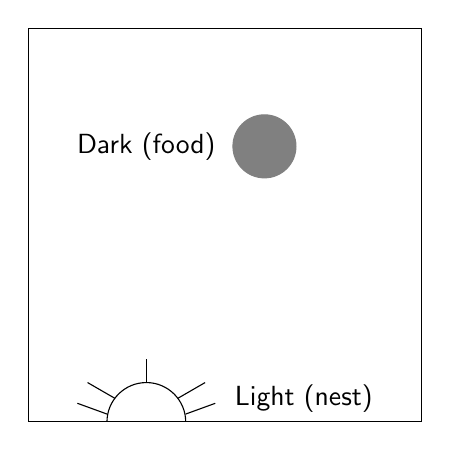
\begin{tikzpicture}
% Light and dark with labels
\draw (0,0) -- (5,0) -- (5,5) -- (0,5) -- cycle;
\draw (2,0) arc[start angle=0, end angle=180, radius=5mm];
\node at (3.5,.3) {\textsf{Light (nest)}};
\draw (19mm,3mm) -- +(30:4mm);
\draw (20mm,1mm) -- +(20:4mm);
\draw (11mm,3mm) -- +(150:4mm);
\draw (10mm,1mm) -- +(160:4mm);
\draw (15mm,5mm) -- (15mm,8mm);
\draw[fill,gray] (3,3.5) circle[radius=4mm];
\node at (1.5,3.5) {\textsf{Dark (food)}};
\path (0,-.1) -- (5,-.1); % To prevent truncation
\end{tikzpicture}
}
\hspace{\fill}
\rightfigure[c]{
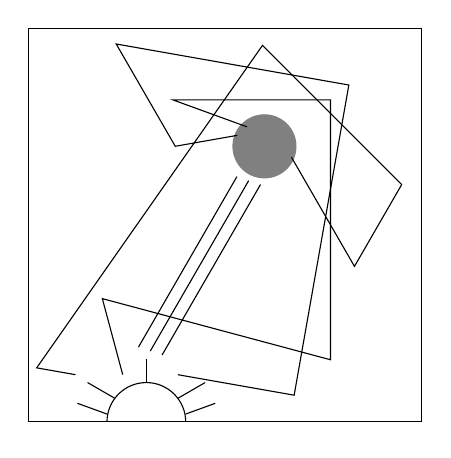
\begin{tikzpicture}
\draw (0,0) -- (5,0) -- (5,5) -- (0,5) -- cycle;
\draw (2,0) arc[start angle=0, end angle=180, radius=5mm];
\draw (19mm,3mm) -- +(30:4mm);
\draw (20mm,1mm) -- +(20:4mm);
\draw (11mm,3mm) -- +(150:4mm);
\draw (10mm,1mm) -- +(160:4mm);
\draw (15mm,5mm) -- (15mm,8mm);
\draw[fill,gray] (3,3.5) circle[radius=4mm];
% Straight lines between light and dark
\begin{scope}[xshift=-1mm,yshift=2mm]
%\draw (13.5mm,8mm) -- +(60:2.5);
\draw (15mm,7.5mm) -- +(60:2.5);
\draw (16.5mm,7mm) -- +(60:2.5);
\draw (18mm,6.5mm) -- +(60:2.5);
\end{scope}
% Random lines between light and dark
\draw (19mm,6mm) -- ++(-10:15mm) -- ++(80:40mm) -- ++(170:30mm) -- ++(-60:15mm) -- ++(10:8mm);
\draw (12mm,6mm) -- ++(-75:-10mm) -- ++(-15:30mm) -- ++(90:33mm) -- ++(180:20mm) -- ++(-20:10mm);
\draw (6mm,6mm) -- ++(170:5mm) -- ++(55:50mm) -- ++(-45:25mm) -- ++(-120:12mm) -- ++(120:16mm);
\path (0,-.1) -- (5,-.1); % To prevent truncation
\end{tikzpicture}
}
\leftcaption{The ants' nest and the food source\label{fig.ant-nest-food}}
\rightcaption{Pheromones create a trail\label{fig.ant-nest-food-trail}}
\end{minipage}
\end{figure}

The ant-like behavior can be implemented by a robot.\label{s.ant-like-algo} Assume that there is a fixed area within which the robot can move. As in Fig.~\ref{fig.ant-nest-food} there is a food source and a nest. The food source will be represented by a dark spot that can be easily detected by a ground sensor on the robot. The proximity sensors of the robot are used to detect the walls of the area. Activity~\ref{act.locate-nest} suggests two methods of representing the nest that depend on what additional sensors your robot has.

\begin{framed}
\act{Locating the nest}{locate-nest}
\begin{itemize}
\item Implement a program that causes the robot to move to the nest no matter where it is placed in the area.
\item Accelerometers: Mount the area on a slope such that one corner, the nest, is at the lowest point of the area. 
\item Light sensor: The nest is represented by a light source that can be detected by the light sensor regardless of the position and heading of the robot. If the light sensor is fixed and can detect light only from a certain direction, the robot will have to rotate to locate the light source.
\end{itemize}
\end{framed}

Simulate the pheromones by covering the area with a sheet of white paper and attaching a black marker to the robot so that it draws a line wherever it moves. A ground sensor detects the marks in the area. Figure~\ref{fig.ant-result} shows the lines resulting from the behavior of a robot running the algorithm. Activity~\ref{act.high-density} asks you to explore the ability of the robot to sense areas which have a high density of lines.

\begin{figure}
\begin{center}
\includegraphics[width=.8\textwidth]{density-map-0}
\end{center}
\caption{A robot simulating pheromones of ants}\label{fig.ant-result}
\end{figure}

\begin{framed}
\act{Sensing areas of high density}{high-density}
\begin{itemize}
\item In Sect.~\ref{s.no-gradient} we noted that sensors don't sense a single geometrical point but rather have an aperture that reads a relatively large area, perhaps even as much as a square centimeter (Fig.~\ref{fig.no-gradient}). Experiment with your ground sensor to see how the readings returned by the sensor depend on the width of the line. Can you come to any conclusion about the optimal width of the marker? If it is too thin the trail won't be detected and if it is too thick the markings of the random movement might be taken to be the trail.
\item Represent the food source as a relatively large totally black spot and make sure that it gives a minimal reading of the ground sensor.
\item Figure~\ref{fig.ant-result} shows that the trail between the food source and the nest has a high density. Experiment with various numbers of lines and define an effective threshold between the trail and areas of random motion outside the trail. See if you can get the robot to make darker lines by varying its motion or by moving back and forth along the trail.
\end{itemize}
\end{framed}

\section{A probabilistic model of the ants' behavior}\label{s.ant-probabilistic}
\index{path finding!probabilistic model of the ants}

A \emph{model} is an abstraction of a system that shows how parameters impact phenomena. Models are used, for example, to study traffic patterns in order to predict the effect of new roads or traffic lights. To understand how the path from the nest to the food is generated, this section presents a simplified model the behavior of the ants. 

The fundamental characteristic of the ants' behavior is that they do not have a map of their environment, so they must move randomly in order to search for the food source. Therefore, a model of their behavior must be probabilistic. Let us assume that the environment is a rectangular area that is a grid of cells. Figure~\ref{fig.ant-grid-empty} shows an area split into $6\times 8=48$ cells.

\begin{quote}
\begin{center}
\textbf{Coordinates in a grid of cells}
\end{center}
Throughout the book, the coordinates of a cell in a grid are given as $(\textit{row}, \textit{column})$. Rows are numbered from top to bottom and columns from left to right like matrices in mathematics, however, the numbering starts from $0$, as in the array data type in computer science.
\end{quote}

\begin{figure}
\begin{center}
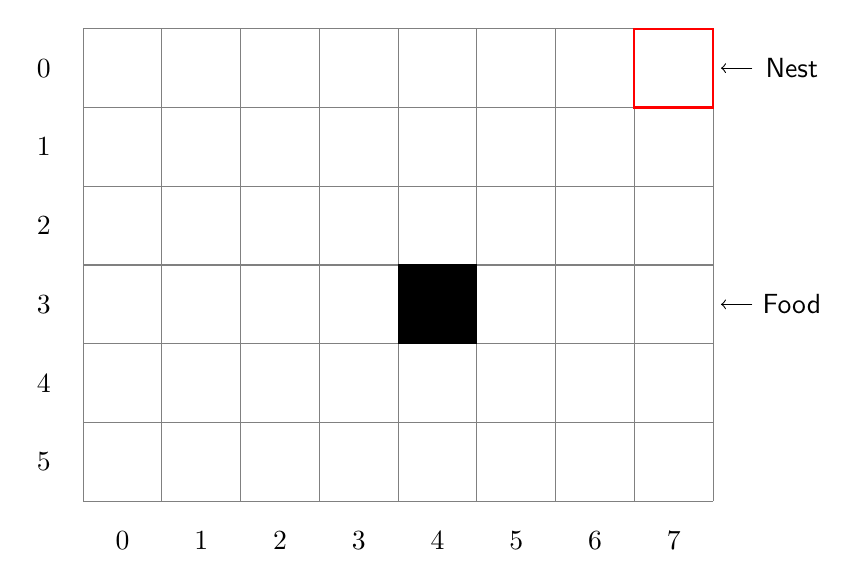
\begin{tikzpicture}
\draw[step=1cm,gray,thin] (0,0) grid (8,6);
\foreach \n/\x in {0/.5, 1/1.5, 2/2.5, 3/3.5, 4/4.5, 5/5.5, 6/6.5, 7/7.5}
  \node at (\x, -.5) {\p{\n}};
\foreach \n/\y in {5/.5, 4/1.5, 3/2.5, 2/3.5, 1/4.5, 0/5.5}
  \node at (-.5, \y) {\p{\n}};
\draw[fill] (4,2) rectangle +(1,1);
\node at (9,2.5) {\textsf{Food}};
\draw[->] (8.5,2.5) to +(-.4,0);
\node at (9,5.5) {\textsf{Nest}};
\draw[->] (8.5,5.5) to +(-.4,0);
\draw[red,thick] (7,5) rectangle +(1,1);
\end{tikzpicture}
\end{center}
\caption{Representation of the environment as a grid of cells}\label{fig.ant-grid-empty}
\end{figure}

Without any information on how ants choose their movements, we assume that they can move in any direction with the same probability, so the probability $p$ of an ant being in any cell is $1$ divided by the number of cells, here $p=1/48=0.021$.

The probability that the ant is in the cell with the food source is $p$, the same as for any other cell. According to our specification of the ant's behavior, once it enters this cell and identifies the cell as the food source, it returns directly to the nest. In Fig.~\ref{fig.ant-grid-empty} the food source is in cell $(3,4)$, so an ant visiting that cell must return to the nest at cell $(0,7)$, passing through cells $(2,5)$ and $(1,6)$. What is the probability that the ant is in any of these three cells? There are two possibilities: either the ant is in the cell because it randomly moved there with probability $p$, or the ant is there because it moved to the food source randomly with probability $p$ and then \emph{with probability $1$} is moved towards the nest. Therefore, the total probability of being in any of those cells is $p+p\times 1=p+p=2p$.\footnote{After the probabilities are updated they must be normalized as explained in Appendix~\ref{a.normalize}. For another example of normalization, see Sect.~\ref{s.prob-local}.}  If our robot is drawing lines as it moves, the cells on the diagonal should be twice as dark as the other cells.

\begin{figure}
\begin{center}
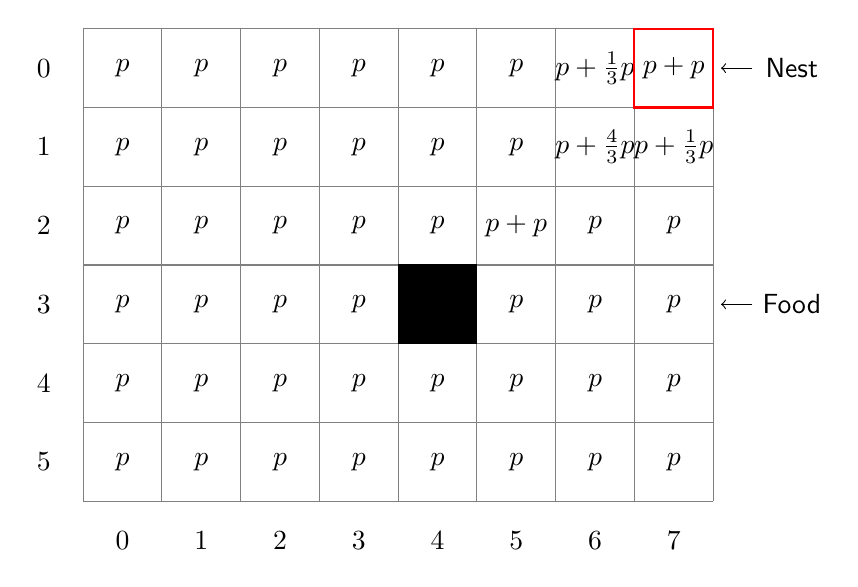
\begin{tikzpicture}
\draw[step=1cm,gray,thin] (0,0) grid (8,6);
\foreach \n/\x in {0/.5, 1/1.5, 2/2.5, 3/3.5, 4/4.5, 5/5.5, 6/6.5, 7/7.5}
  \node at (\x, -.5) {\p{\n}};
\foreach \n/\y in {5/.5, 4/1.5, 3/2.5, 2/3.5, 1/4.5, 0/5.5}
  \node at (-.5, \y) {\p{\n}};
\draw[fill] (4,2) rectangle +(1,1);
\node at (9,2.5) {\textsf{Food}};
\draw[->] (8.5,2.5) to +(-.4,0);
\node at (9,5.5) {\textsf{Nest}};
\draw[->] (8.5,5.5) to +(-.4,0);
\foreach \x in {.5, 1.5, 2.5, 3.5}
  \foreach \y in {.5, 1.5, 2.5, 3.5, 4.5, 5.5}
     \node at (\x,\y) {$p$};
\foreach \y in {.5, 1.5, 3.5, 4.5, 5.5}
     \node at (4.5,\y) {$p$};
\foreach \y in {.5, 1.5, 2.5, 4.5, 5.5}
     \node at (5.5,\y) {$p$};
\foreach \x in {6.5, 7.5}
  \foreach \y in {.5, 1.5, 2.5, 3.5}
     \node at (\x,\y) {$p$};
\node at (5.5,3.5) {$p+p$};
\node at (7.5,5.5) {$p+p$};
\node at (6.5,4.5) {$p+\frac{4}{3}p$};
\node at (7.5,4.5) {$p+\frac{1}{3}p$};
\node at (6.5,5.5) {$p+\frac{1}{3}p$};
\draw[red,thick] (7,5) rectangle +(1,1);
\end{tikzpicture}
\end{center}
\caption{Probabilities for the location of the ant}\label{fig.ant-grid-prob}
\end{figure}

\begin{figure}
\begin{center}
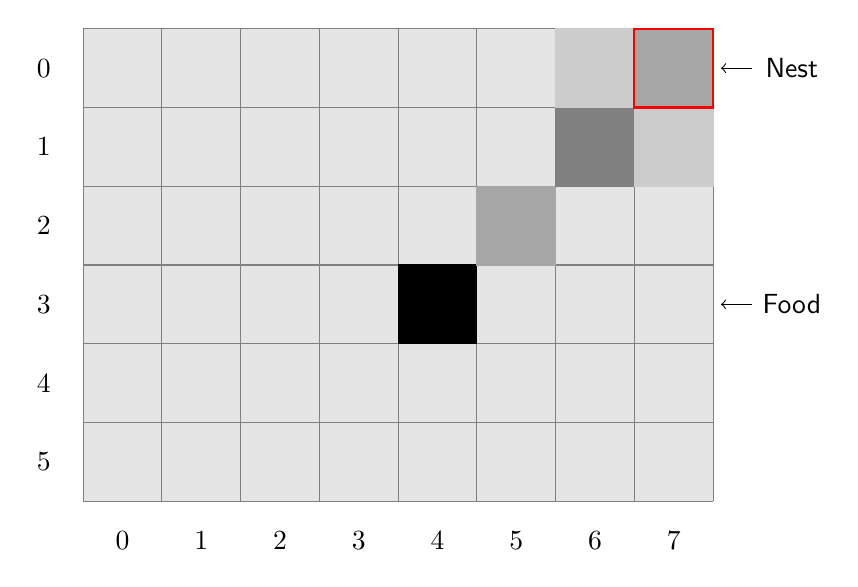
\begin{tikzpicture}
\node at (9,2.5) {\textsf{Food}};
\draw[->] (8.5,2.5) to +(-.4,0);
\node at (9,5.5) {\textsf{Nest}};
\draw[->] (8.5,5.5) to +(-.4,0);
\foreach \x in {0, 1, 2, 3, 4, 5, 6, 7}
  \foreach \y in {0, 1, 2, 3, 4, 5}
  \draw[fill,gray!20] (\x,\y) rectangle +(1,1);
\draw[step=1cm,gray,thin] (0,0) grid (8,6);
\draw[fill] (4,2) rectangle +(1,1);
\draw[fill,gray!70] (5,3) rectangle +(1,1);
\draw[fill,gray] (6,4) rectangle +(1,1);
\draw[fill,gray!70] (7,5) rectangle +(1,1);
\draw[fill,gray!40] (6,5) rectangle +(1,1);
\draw[fill,gray!40] (7,4) rectangle +(1,1);
\foreach \n/\x in {0/.5, 1/1.5, 2/2.5, 3/3.5, 4/4.5, 5/5.5, 6/6.5, 7/7.5}
  \node at (\x, -.5) {\p{\n}};
\foreach \n/\y in {5/.5, 4/1.5, 3/2.5, 2/3.5, 1/4.5, 0/5.5}
  \node at (-.5, \y) {\p{\n}};
\draw[red,thick] (7,5) rectangle +(1,1);
\end{tikzpicture}
\end{center}
\caption{Probabilities for the location of a robot with a marker}\label{fig.ant-grid-gray}
\end{figure}

Once the ant has reached the nest, it will move randomly again, that is, it will select a random neighbor to move to. In general a cell has eight neighbors (above and below, left and right, four on the diagonals), so the probability is $p/8$ that it will be in any one of these neighbors. The nest, however, is in the corner with only three neighbors, so the probability is $p/3$ that it will move to any one of them. Figure~\ref{fig.ant-grid-prob} shows the probability of the location of the ant after finding the food source, returning to the nest and making one additional random move. When implemented by a robot with a marker, the cells with higher probability will become darker (Fig.~\ref{fig.ant-grid-gray}).

What can we conclude from this model?
\begin{itemize}
\item Although the ants move randomly, their behavior of returning to the nest after finding the food source causes the probability of being on the diagonal to be higher than anywhere else in the environment. 
\item Since the ants drop pheromones (black marks) at every cell they visit, it follows that the marks on the diagonal path between the food source and the nest will be darker than the marks on other cells. Eventually, the markings on this path will be sufficiently dark so that the robot can follow it to the food source without performing a random exploration.
\item Since the robot visits the nest often, the cells in the immediate vicinity of the nest will have a probability somewhere between the uniform probability and the high probability of the trail. Therefore, it is important to emphasize the trail using methods such as those explored in Activity~\ref{act.high-density}.
\end{itemize}

\section{A finite state machine for the path finding algorithm}\label{s.fsm-ants}
\index{path finding!ants}

An FSM for path finding by the ants is shown in Fig.~\ref{fig.fsm-ant}. To save space the labels of the transitions use abbreviations which are explained in Table~\ref{tab.abbrev}. Here is a detailed description of the behavior specified by this FSM in each state:

\smallskip

\begin{figure}
\begin{center}
\begin{tikzpicture}[node distance = 3.5cm and 4.9cm,align=left,minimum size=14mm,every loop/.style={min distance=16mm}]
% Nodes
\node[draw,circle] (search) {\p{search}};
\node[draw,circle] (follow) [right=of search] {\p{follow}};
\node[draw,circle] (food) [below=of follow] {\p{at food}};
\node[draw,circle] (nest) [below=of search] {\p{goto}\\\p{nest}};
% Initial state arrow
\draw[->] (-15mm,10mm) to node [above left,xshift=6pt] {\p{true} $\leadsto$ \p{fwd}} (search);
% Transitions from search
\path[->] (search) edge [loop left] node [below,yshift=-1mm] {\p{wall} $\leadsto$\\\p{turn $90$--$270$,}\\\p{fwd}} ();
\path[->] (search) edge [loop above] node {\p{timeout} $\leadsto$\\\p{turn $0$--$360$,}\\\p{fwd}} ();
\path[->,bend left=40] (search) edge node[above,xshift=-2mm,yshift=-3mm] {\p{gray} $\leadsto$  \p{fwd}} (follow);
% Transitions from follow
\path[->] (follow) edge [loop above] node[yshift=-1mm] {\p{gray R/L} $\leadsto$\\\p{fwd R/L}} ();
\path[->] (follow) edge [loop right] node [below,yshift=-1mm,xshift=-3mm] {\p{gray R\&L} $\leadsto$\\\p{fwd}} ();
\path[->] (follow) edge node[above,yshift=-3mm] {\p{timeout} $\leadsto$ \p{fwd}} (search);
\path[->,bend left=15] (follow) edge node[left,yshift=4mm,xshift=17mm] {\p{black} $\leadsto$ \p{--}} (food);
\path[->,bend left=40] (follow) edge node[below,xshift=4mm] {\p{wall} $\leadsto$\\\p{turn} $450$--$360$, \p{fwd}} (search);
% Transitions from at food
\path[->] (food) edge [loop right] node [below,yshift=-3mm,xshift=-2mm] {\p{nest direction}\\\p{not found} $\leadsto$\\\p{rotate}} ();
\path[->] (food) edge node[below,yshift=2mm] {\p{nest direction found} $\leadsto$\\\p{turn to nest}} (nest);
% Transitions from nest
\path[->,bend left=15] (nest) edge node[right,xshift=-23mm,yshift=1mm] {\p{at nest} $\leadsto$ \p{fwd}} (search);
\path[->] (nest) edge [loop left] node [above,yshift=1mm] {\p{nest R/L} $\leadsto$\\\p{fwd R/L}} ();
\path[->] (nest) edge [loop below] node[left,xshift=-8mm,yshift=4mm] {\p{nest front} $\leadsto$\\\p{fwd}} ();
\end{tikzpicture}
\end{center}
\caption{State machine for drawing a path between a food source and a nest\newline See Table~\ref{tab.abbrev} for explanations of the abbreviations}\label{fig.fsm-ant}
\end{figure}

\begin{table}[bt]
\caption{Abbreviations in the state machine}
\label{tab.abbrev}
\begin{tabular}{p{2.5cm}p{8cm}}
\svhline\noalign{\smallskip}
Abbreviation & Explanation \\
\noalign{\smallskip}\svhline\noalign{\smallskip}
\p{fwd} & \p{set motor forwards}\\
\p{fwd R/L} & \p{set motor forwards and to the right/left}\\
& \p{\bfseries fwd and fwd R/L also set the timer to a random period}\\
\p{wall} & \p{wall detected}\\
\p{timeout} & \p{timer period expired}\\
\p{gray R/L/R\&L} & \p{gray detected by right/left/both sensors}\\
\p{nest front/R/L} & \p{nest detected in front/right/left}\\
\p{black} & \p{black detected}\\
\p{nest direction} & \p{direction from food to nest found or not found}\\
\p{turn $\theta_1$--$\,\theta_2$} & \p{turn randomly in the range $\theta_1$--$\,\theta_2$}\\
\p{rotate}&\p{the robot (or its sensor) rotates}\\
\noalign{\smallskip}\svhline\noalign{\smallskip}
\end{tabular}
\end{table}

\noindent\textbf{\p{search}:} In this state the robot randomly searches for dark areas. It is the initial state and the transition \p{true $\leadsto$ fwd} specifies that initially (and unconditionally) the robot is moving forwards and a timer is set to a random period. When the timer expires (\p{timeout}), the robot makes random turn, moves forwards and resets the timer. This random motion will continue until the robot encounters the wall of the area or a gray marking on the surface of the area. If it encounters a wall it makes a random turn \emph{away} from the wall; we assume that the sensor faces directly ahead so the random turn must be in some direction to the side or the rear of the robot. Once the robot has detected a gray marking, it makes the transition to the \p{follow} state.

\smallskip

\noindent\textbf{\p{follow}:} The two self-transitions above and to the right of this state are transitions that implement line following (Sect.~\ref{s.line}). There are three other transitions: Should a \p{timeout} occur without detecting gray, the robot is no longer following a line and must return to the \p{search} state. If the robot encounters a wall, we want it to turn away, but first we ask it to make a full $360^\circ$ turn to check if there is a gray marking in its vicinity. Therefore, the transition includes the action \p{turn} $450$--$360$. Since the nest is next to a wall, this condition is also true when the robot returns to the nest. If the robot senses a high-density marking (\p{black}), it concludes that it has reached the food source and takes the transition to the state \p{at food}.

\smallskip

\noindent\textbf{\p{at food}:} Finally, the robot has discovered the food source. It must now return to the nest. We specified that the nest can be detected (Activity~\ref{act.locate-nest}), but the robot's sensor does not necessarily face the direction of the nest. Therefore, the robot (or its sensor) must rotate until it finds the direction to the nest. When it does so, it turns towards the nest and takes the transition to the state \p{goto nest}.

\smallskip

\noindent\textbf{\p{goto nest}:} This state is similar to the \p{follow} state in that the robot moves forward towards the nest, turning right or left as needed to move in the direction of the nest. When it reaches the nest it returns to the \p{search} state.

\smallskip

Look again at Fig.~\ref{fig.ant-result} which shows an actual experiment with a robot running this algorithm. We see that there is a high density of lines between the nest and food source, but there is also a relatively high density of lines in the vicinity of the nest, not necessarily in the direction of the food source. This can cause to robot to return to random searching instead of going directly to the food source.

\section{Summary}

The obstacle avoidance algorithms use wall following algorithms that have been known since ancient times in the context of navigating a maze. When used for obstacle avoidance, various anomalies can cause the algorithms to fail, in particular, the $G$-shaped obstacle can trap a wall following algorithm. The Pledge algorithm overcomes this difficulty.

A colony of ants can determine a path between their nest and a food source without knowing their location and without a map by reinforcing random behavior that has a positive outcome.

\section{Further reading}

There is a large literature on mazes that can be found by following the references in the Wikipedia article for \emph{Maze}. The Pledge algorithm was discovered by 12-year-old John Pledge; our presentation is based on \cite[Chap.~4]{turtle}. A project based on ants following pheromones is described in~\cite{Mayet2010}.


\bibliographystyle{spmpsci}
\bibliography{er}
